\chapter{Appendix}

\section{Appendix A - Chapter 4}

\section{Appendix B - Chapter 5}

\begin{figure}[t]
\centering
\includegraphics[scale=0.12]{figures/t-sne halpha masked with cotar.png}
\caption{t-SNE map for all spectra in DR3 with H$\upalpha$ emission-line spectra identified by Čotar et al. tagged in pink.}
\label{fig5.3}
\end{figure}

\begin{figure}[t]
\centering
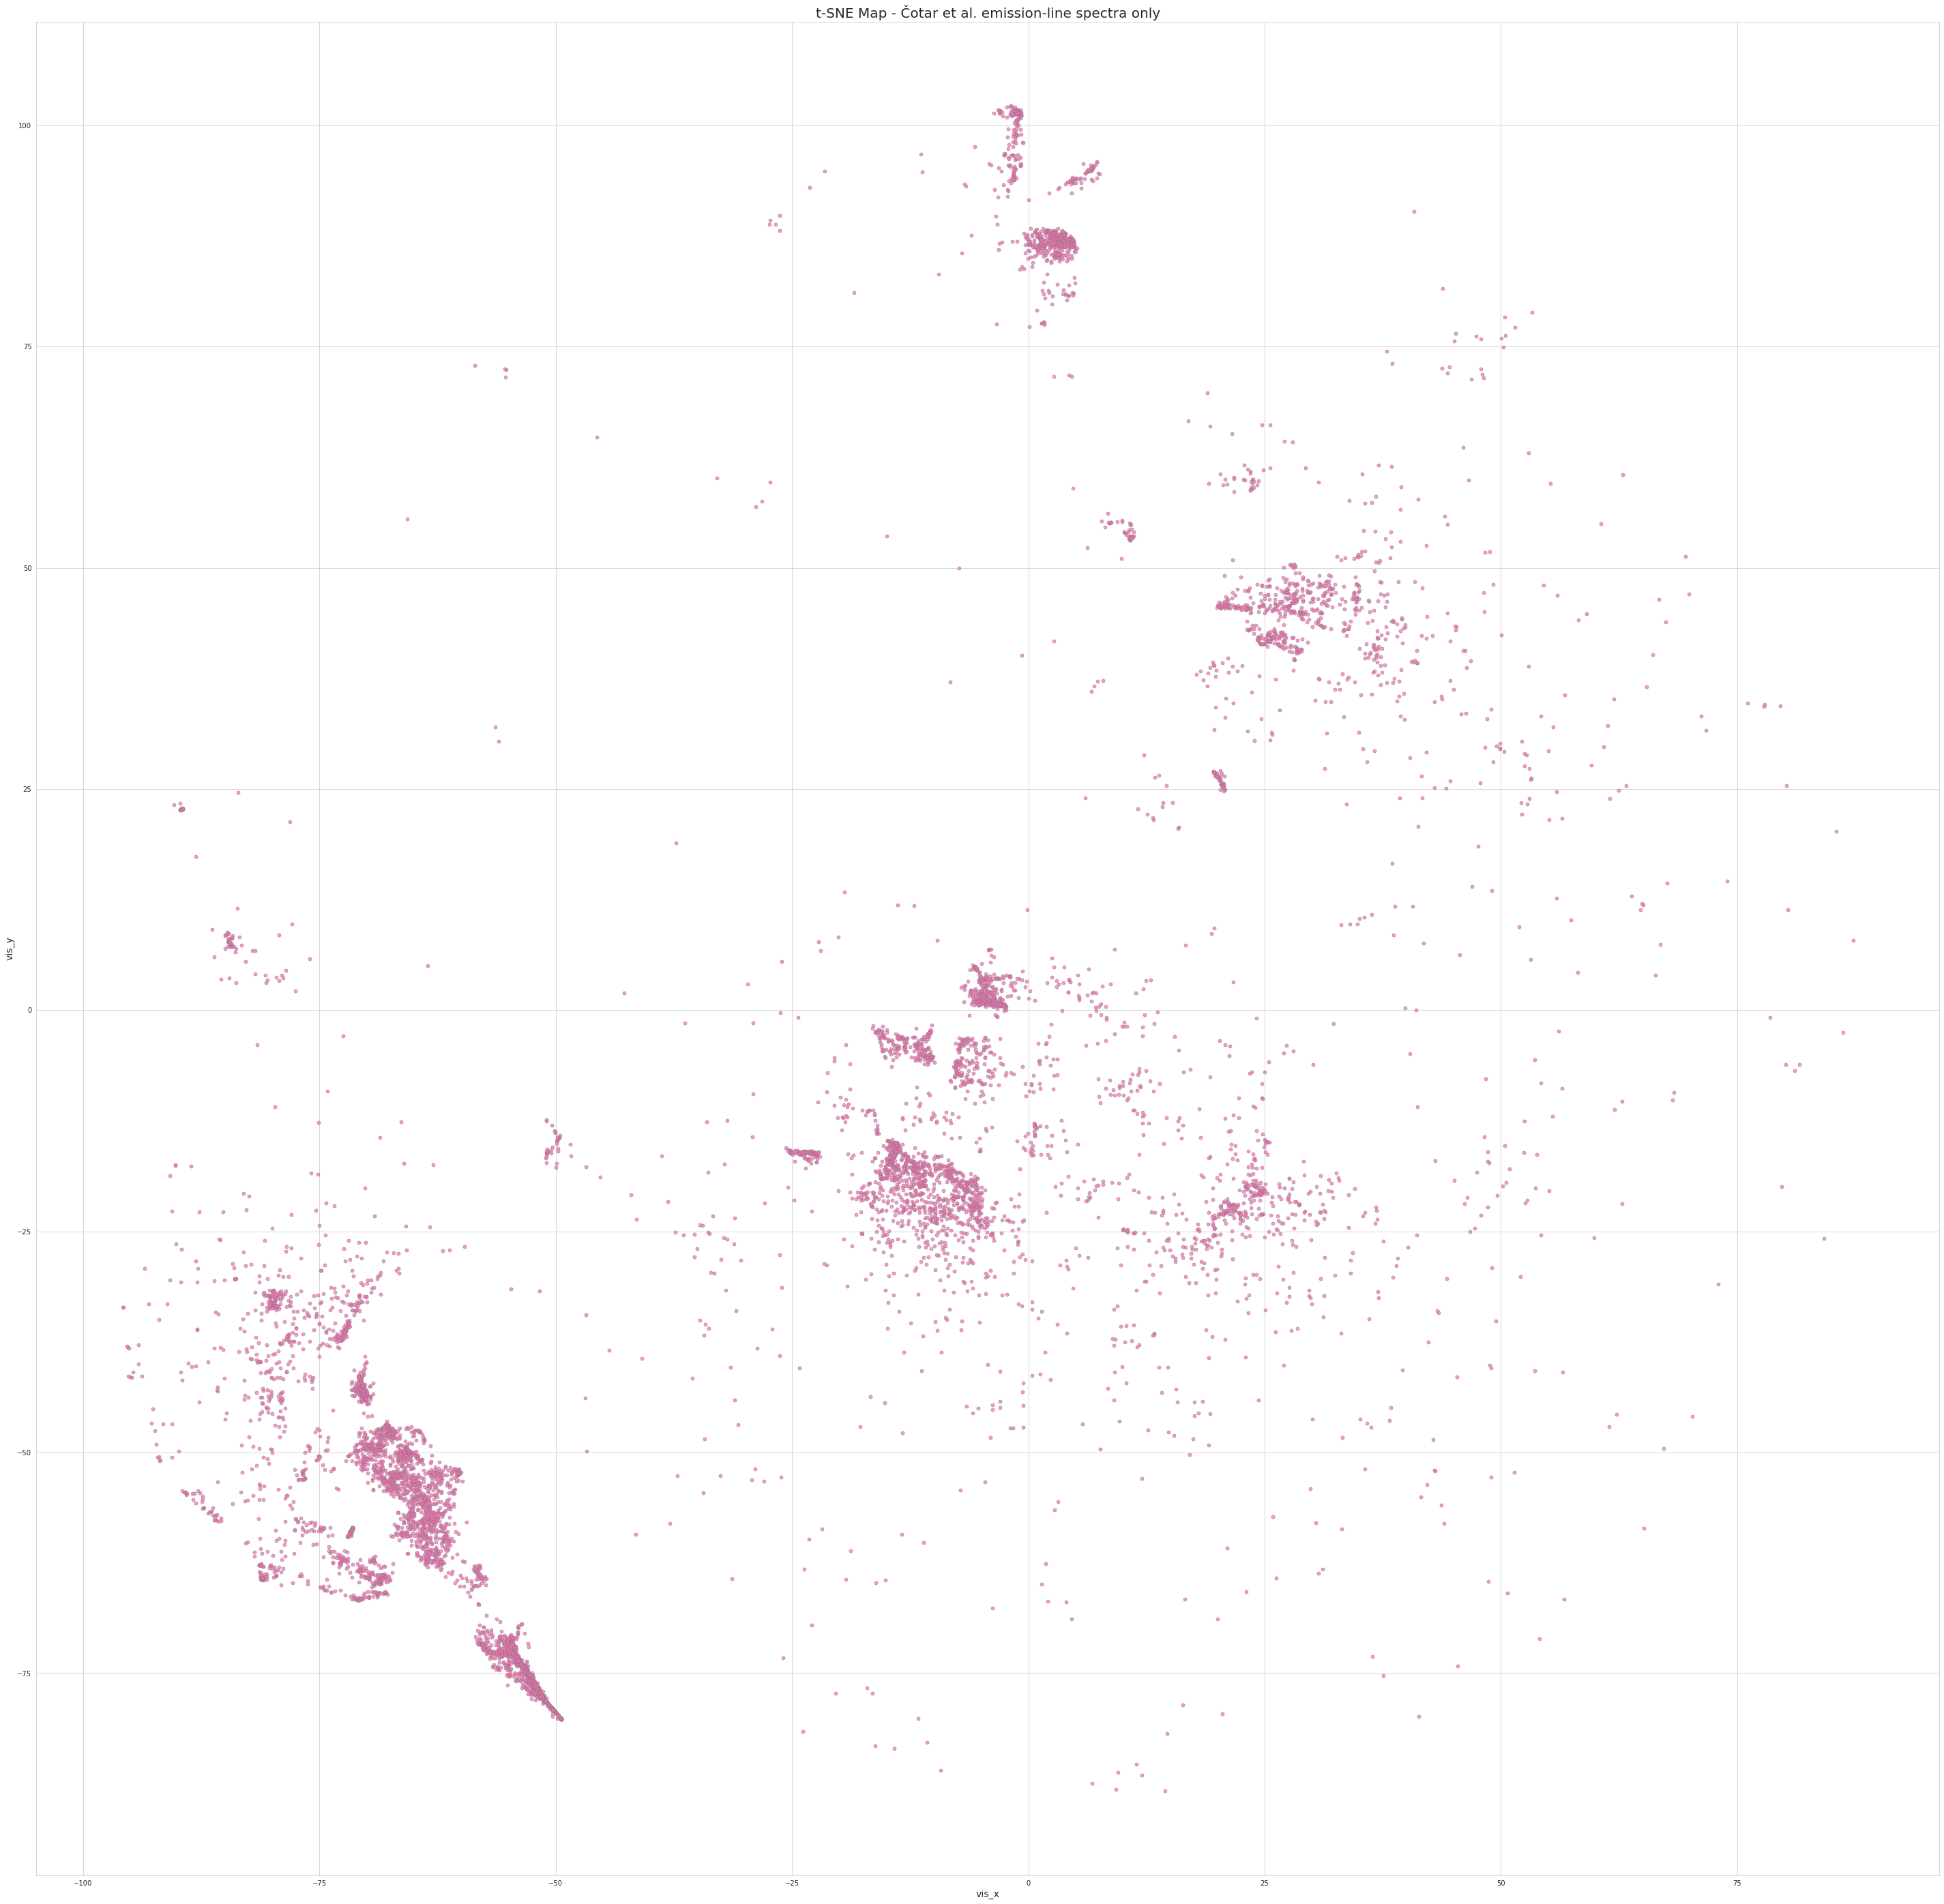
\includegraphics[scale=0.12]{figures/tsne_cotar_only.png}
\caption{H$\upalpha$ emission-line spectra identified by Čotar et al. projected to the same t-SNE map, excluding presumably typical spectra.}
\label{fig5.3}
\end{figure}

\section{Appendix C - Chapter 6}

\begin{table}[!htb]
\begin{center}
\begin{tabular}{|l|l|}
\hline
\textbf{count} & 7067.000000 \\ \hline
\textbf{mean} & 0.532952 \\ \hline
\textbf{std} & 0.444046 \\ \hline
\textbf{min} & 0.220042 \\ \hline
\textbf{25\%} & 0.280778 \\ \hline
\textbf{50\%} & 0.388232 \\ \hline
\textbf{75\%} & 0.562633 \\ \hline
\textbf{max} & 5.055410 \\ \hline
\end{tabular}
\caption{EW distribution summary statistics for emission-line stars identified in GALAH DR3}
\label{table:draglift1}
\end{center}
\end{table}

\begin{table}[!htb]
\begin{center}
\begin{tabular}{|l|l|}
\hline
\textbf{count} & 10364.000000 \\ \hline
\textbf{mean} & 0.539950 \\ \hline
\textbf{std} & 0.420590 \\ \hline
\textbf{min} & 0.250070 \\ \hline
\textbf{25\%} & 0.298572 \\ \hline
\textbf{50\%} & 0.392470 \\ \hline
\textbf{75\%} & 0.592625 \\ \hline
\textbf{max} & 5.369496 \\ \hline
\end{tabular}
\caption{EW distribution summary statistics for emission-line stars identified by Čotar et al. (various surveys).}
\label{table:draglift1}
\end{center}
\end{table}

\begin{figure}[!htb]
\centering
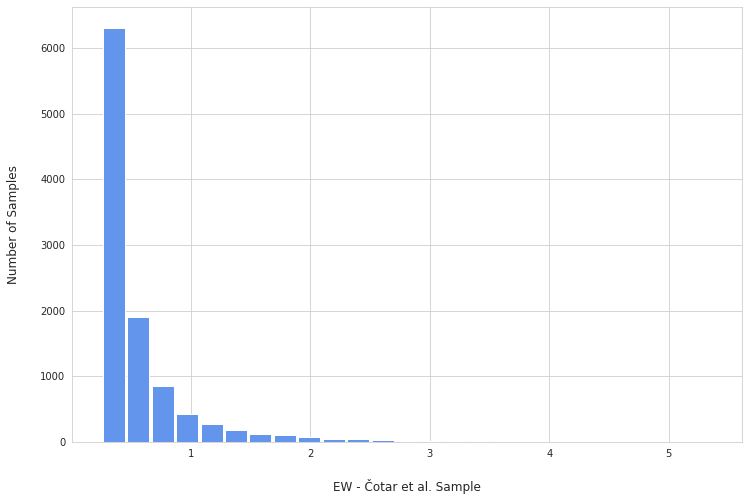
\includegraphics[scale=0.50]{figures/EW hist cotar.png}
\caption{The equivalent width (EW) distribution of the inverted difference spectra of the emission-line spectra provided by Čotar et al. Here EW > 0.25. Note that this sample contains additional spectra not in GALAH DR3.}
\end{figure}

